\chapter{Background}
\label{cha:background}

Sectra AB is creating products both in medical IT and secure communications.
It is a multinational corporation that currently has offices in 12 countries.
Medical imaging is their biggest business, and radiology is the main area within that.
They are currently pursuing a research project with Region Skåne.
Region Skåne is responsible for the healthcare in Skåne, the southern most county of Sweden.
The goal behind the project is to use machine learning and text mining techniques to improve the functionality of their products and aid the physicians in their work.
Among other things, this can be suggesting categories to doctors while they are writing medical reports.
Another case is to use the categories of documents to present doctors with medical reports that are dealing with similar cases from the past.
With this information the doctors could get an extra quality assurance check in their diagnostic flow.

By using machine learning techniques there are plenty of opportunities and ways to accomplish new interesting things with textual data.
But in order to build these system, you need a substantial amount of clinical reports that are labeled.
Therefore, the purpose of this thesis is to increase the quality and efficiency of the process of labeling these reports.
This will be done by using unsupervised learning techniques such as topic models to first remove invalid reports that are not supposed to be labeled.
These are documents that describe patients that did not get examined for some reason.
Examples of this can be deceased patients, patients being moved to a different hospital or simply patients that cancelled their appointments.

For the process of labeling the reports, a complete system is needed.
This system should use active learning in conjunction with the aforementioned unsupervised techniques to increase the quality of the labeled documents.
In the work that they have done so far in the research project a doctor has done some initial labeling of reports.
This was done by simply selecting the reports in the order they were on file.
The doctor that primarily worked with the labeling stated that the distribution over the labeled categories was very skewed.
The vast majority of labeled documents were assigned to a small subset of the categories.
In addition, a skewed dataset causes the number of clinical reports that need to be labeled to increase a lot.
For a statistical model to be able to achieve good results with the less frequently occurring categories, a large number of reports needs to be labeled in order to obtain a good amount of reports with these categories.

By using active learning, that is active selection of the samples to be labeled, the goal is to reduce the number of labeled samples needed to achieve sufficient results with the model.
Sectra has a simple website that they use for labeling reports, which the active learning techniques will be incorporated into.
The existing web interface can be seen in Figure~\ref{fig:web-interface}.

\begin{figure}
      \centering
      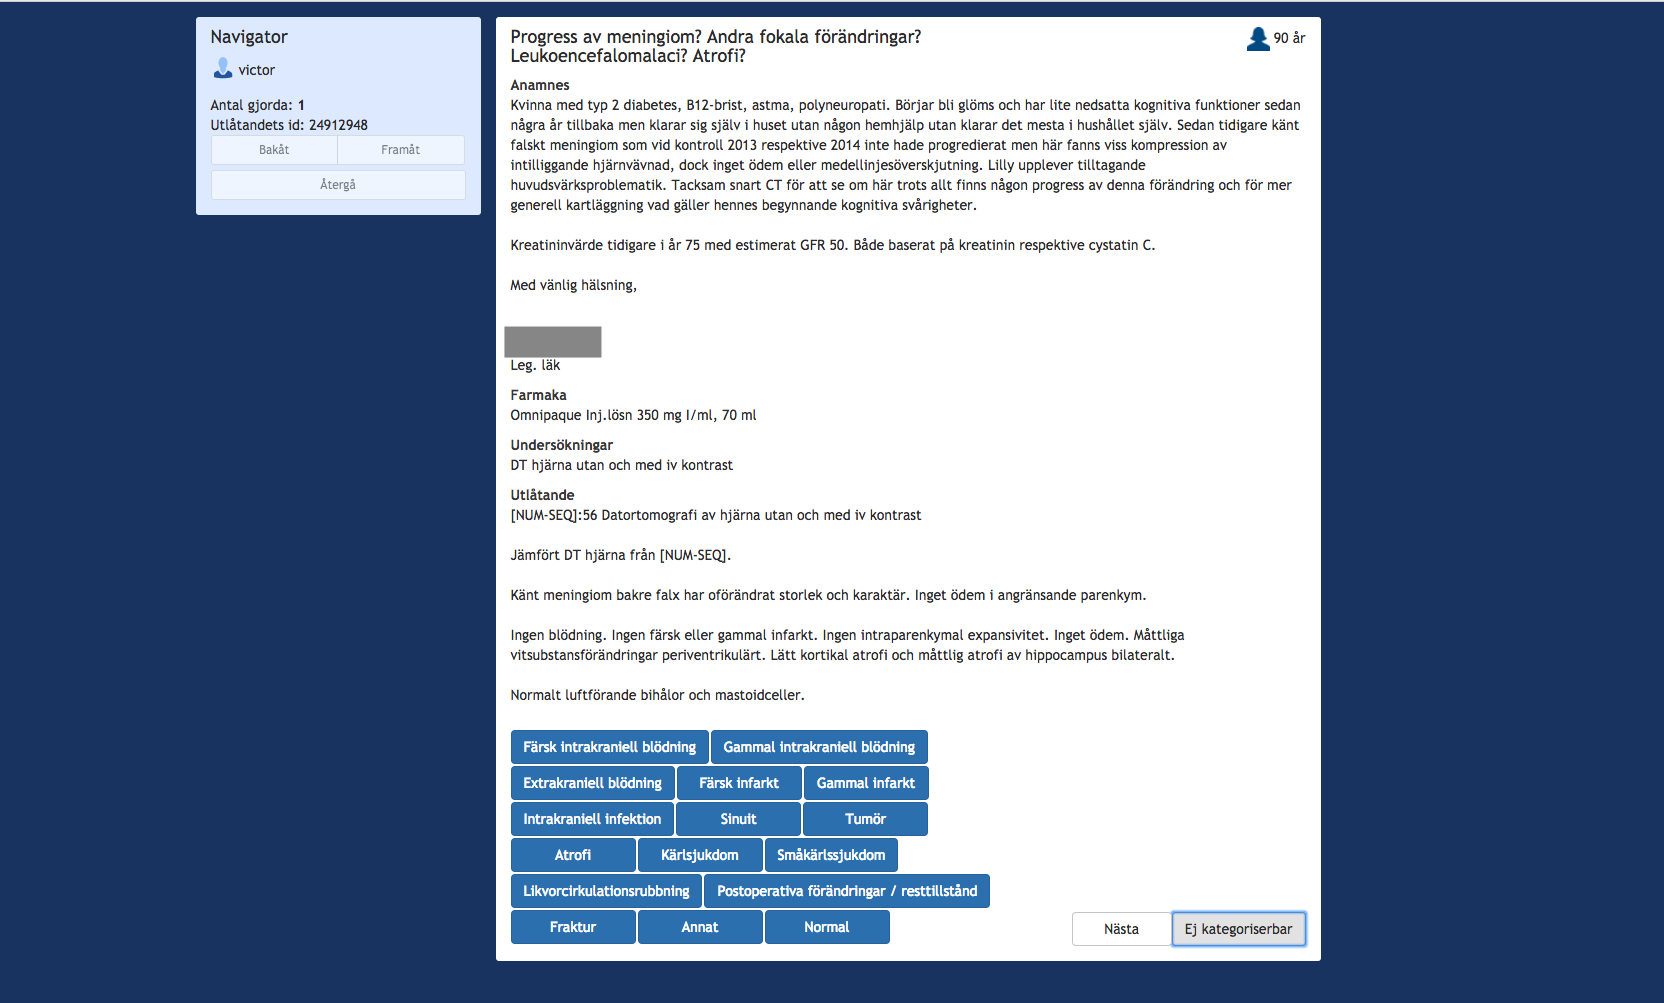
\includegraphics[scale=0.25]{web-interface}
      \caption{A screenshot of the interface used to label clinical reports at Sectra}
      \label{fig:web-interface}
\end{figure}
